\documentclass[a4paper, 12pt]{article}
\usepackage{mathtools}
\usepackage{bm}
\usepackage{tikz}
\usepackage{float}
\usepackage{pgfplots}
\setlength{\parindent}{0cm}
\setlength{\parskip}{12pt plus4mm minus3mm}

\usepgfplotslibrary{units}

\begin{document}
\section{The motion of the polhode}
Given a rigid rotating object, with angular momentum $L$ and kinetic energy $T$, let us work in a rotating reference frame moving with the object. In that frame we will use Cartesian co-ordinates aligned with the three principal axes of the moment of inertia of the object.

In those co-ordinates let the angular velocity vector $\bm{\omega}$ have components $\omega_1, \omega_2,\omega_3$. The moment of inertia tensor $\bm{I}$ has the form:

$$
I = \begin{pmatrix}
I_1 & 0 & 0 \\
0   & I_2 & 0 \\
0 & 0 & I_3 \\  
\end{pmatrix}
$$

We will assume all principal axes are distinct and that (for the sake of argument) $I_1 < I_2 < I_3$. We will refer to the unit vectors in this co-ordinate system as $\bm{n_1}, \bm{n_2}, \bm{n_3}$.

The inertia tensor may be visualised using an ellipsoid. In 3D space, consider the surface traced out by the vector $\bm{x}$ subject to the constraint $\bm{x}\cdot\bm{I}\cdot\bm{x} = 1$. This is an ellipsoid with equation $$I_1x^2 + I_2y^2 + I_3z^2 = 1$$

For fixed angular momentum (in a situation where there is no torque) $\bm{I}\cdot\bm{\omega}$ is constant and hence the magnitudes of $I$  and $\omega$ are inversely proportional. Kinetic energy is given by $\frac{\bm{I}\cdot\bm{\omega}^2}{2}$. It will be at a minimum where $\omega$ is least and hence when $I$ is largest, which is when the axis of rotation is pointing in the direction of $\bm{n_3}$. Similarly the energy is at a maximum where the axis of rotation is pointing in the direction of $\bm{n_1}$.

Informally, for the same angular momentum, reducing the moment of inertia about an axis will proprtionately increase the angular velocity. The kinetic energy depends will decrease linearly with the moment of inertia (because the mass of the object is closer in and so less of it is rotating at the higher speeds on the outer edge of the object) but increase as the square of the angular velocity. The result is that the lower the moment of inertia, the higher the kinetic energy for any given angular momentum.

Exactly the same reasoning shows that the situation is the other way around when considering possible angular moment for constant kinetic energy. The minimum angular momentum will be in the direction of $\bm{n_1}$ and the maximum in the direction of $\bm{n_3}$.

This, and many other things, should be clearer if we may consider two ellipsoids traced out by the angular velocity vector:
\begin{itemize}
\item The {\bf energy ellipsoid} or {\bf Poinsot's ellipsoid}, representing a surface of constant kinetic energy. This is congruent to the inertia ellipsoid but scaled up by a factor of $T$.
  \begin{equation}\label{eq:energy_ellipsoid}
    I_1\omega_1^2 + I_2\omega_2^2 + I_3\omega_3^2 =T
  \end{equation}
\item The {\bf momental ellipsoid}, representing a surface of constant angular momentum. This will in general have a different shape from the inertia ellipsoid.
  \begin{equation}\label{eq:momental_ellipsoid}
    I_1^2\omega_1^2 + I_2^2\omega_2^2 + I_3^2\omega_3^2 = L^2
  \end{equation}
\end{itemize}

In the general case of distinct principal axes of the moment of inertia tensor that we are considering these two ellipsoids will be different shapes. The energy ellipsoid's maximum and minimum lengths will be along the first and third axes respecitvely, whereas the momental ellipsoid will bulge the other way, with the third axis being the longest and the first shortest.

%A specific example may help. The Swan Vesta matchbox is particularly well suited to angular momentum problems because of its dimensions which are:
%
%\begin{center}
%  \begin{tabular}{l l}
%    height & 17.4mm \\
%    width & 47.68mm \\
%    depth & 79.37mm \\
%  \end{tabular}
%\end{center}
%
%Assuming a mass of roughly $16g$ and a thickness of the box of mm this would give us a moment of inertia tensor (in $\textup{kgcm}^2$) of
%
%$$
%I=
%\begin{pmatrix}
%  1279 & 0 & 0 \\
%  0 & 1788 & 0 \\
%  0 & 0 & 2122 \\
%\end{pmatrix}
%$$

By setting $\omega_1=1$ and $\omega_2=\omega_3=0$ in (\ref{eq:momental_ellipsoid}) we can find the maximum value of the moment of inertia for fixed kinetic energy $T$ and a similar operation find the mimimum:

\begin{eqnarray*}
  I_1T \leq L^2 \leq I_3 T \\
  L^2=I_1T & \textrm{at} & \mathbf{\omega}=(\sqrt{\frac{T}{I_1}}, 0, 0) \\
  L^2=I_3T & \textrm{at} & \mathbf{\omega}=(0, 0, \sqrt{\frac{T}{I_3}}) \label{eq:maxlvalue}\\
\end{eqnarray*}

We shall consider only the situation where there is no external turning force (torque) and no loss of energy (dissipation) both $L^2$ and $T$ are constants. The polhode is constrained to move on the intersection of the two ellipsoids, which will be a single 1-dimensional path in the general case.

\section{Visualising the valid paths}

\pgfmathsetmacro{\I}{1.0}
\pgfmathsetmacro{\J}{4.0}
\pgfmathsetmacro{\K}{11.0}
\pgfmathsetmacro{\T}{20.0}

To help visualise this, we will work with the energy ellipsoid (though exactly the same approach would work for the momental ellipsoid). Consider the projection of the energy ellipsoid onto the plane normal to the first principal axis. The path of the particle can be obtained by eliminating $\omega_1$ from the ellipsoid equations by subtracting $I_1(\ref{eq:energy_ellipsoid})$ from $(\ref{eq:momental_ellipsoid})$.

\begin{align}
  (I_2^2 - I_1I_2)\omega_2^2 + (I_3^2-I_1I_3)\omega_3^2 & = L^2 - I_1T\label{eq:momell23}
\end{align}

Because $I_1$ is smaller than both $I_2$ and $I_3$ the coefficients of $\omega_1$ and $\omega_2$ are both positive. The RHS is also positive because $L^2 > I_1T$. This is the equation of an ellipse.

\begin{figure}[H]
  
  \begin{center}
    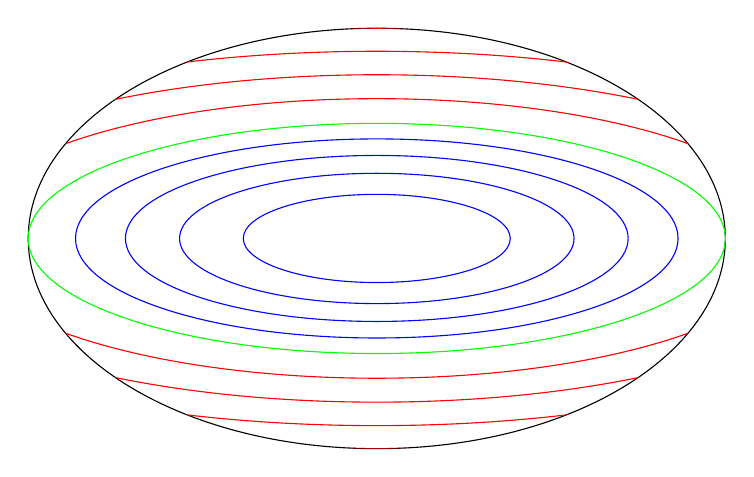
\begin{tikzpicture}[scale=1.4]%[yscale=1.8]%[scale=3]
      \draw [black] (0, 0) ellipse (3.162cm and 1.907cm);
\draw [blue] (0, 0) ellipse (0.000cm and 0.000cm);
\draw [blue] (0, 0) ellipse (1.211cm and 0.400cm);
\draw [blue] (0, 0) ellipse (1.789cm and 0.591cm);
\draw [blue] (0, 0) ellipse (2.280cm and 0.753cm);
\draw [blue] (0, 0) ellipse (2.733cm and 0.903cm);
\draw [green] (0, 0) ellipse (3.162cm and 1.044cm);
\begin{scope}
\clip (0, 0) ellipse (3.162cm and 1.907cm);
\draw [red] (0, 0) ellipse (3.841cm and 1.268cm);
\draw [red] (0, 0) ellipse (4.497cm and 1.485cm);
\draw [red] (0, 0) ellipse (5.140cm and 1.698cm);
\draw [red] (0, 0) ellipse (5.774cm and 1.907cm);
\end{scope}

    \end{tikzpicture}
  \end{center}
  \caption{Projection normal to the first axis}
  \label{fig:proj1}
\end{figure}


Figure \ref{fig:proj1} shows in black the projection of the energy ellipsoid onto the plane normal to $\bm{n_1}$. The coloured ellipses are projections of angular momentum contour lines. 

The blue lines represent angular momentum $L^2\leq I_2T$. The green lines represents angular moment at exactly $L^2=I_2T$. At this point ... the axis of rotation would be entirely about $\bm{n_2}$ ($\bm{\omega}^T=(0, 1, 0)$). These contour lines may be entirely projected within the ``shadow'' of the energy ellipsoid. 

The red lines represent angular momentum $I > I_2T$. Here the contours pass ``behind'' the ellipsoid. Only an arc of an ellipse is projected. The motion of the polhode would appear (in projection) to move backwards and forwards along the arc.

Using the same technique to project from $\bm{n_2}$ tells a different story. Eliminating $\omega_2$ from the ellipsoid equations by subtracting $I_2(\ref{eq:energy_ellipsoid})$ from $(\ref{eq:momental_ellipsoid})$.

\begin{align}
  (I_1^2 - I_1I_2)\omega_1^2 + (I_3^2-I_2I_3)\omega_3^2 & = L^2 - I_2T\label{eq:momell13}
\end{align}

Here $L^2 - I_2T$ and $I_3^2-I_2I_3$ are still positive but $I_1^2 - I_1I_2$ is negative. This is the equation of a hyperbola unless $L^2=I_2T$ in which case it represents two intersecting lines.

\begin{tikzpicture}
\pgfmathsetmacro{\Imax}{sqrt(\T/\I)}
\pgfmathsetmacro{\Kmax}{sqrt(\T/\K)}
    \begin{axis}[
        xlabel={$\omega_2$},
        ylabel={$\omega_1$},
        xmin=-\Imax,xmax=\Imax,
        ymin=-\Kmax,ymax=\Kmax]
        \addplot [red,thick,domain=-\Imax:\Imax] ({sinh(x)}, {cosh(x)});
        \addplot [red,thick,domain=-\Kmax:\Kmax] ({sinh(x)}, {-cosh(x)});
        \addplot[green,dashed] expression {x};
        \addplot[green,dashed] expression {-x};
    \end{axis}
\end{tikzpicture}

\section{Dynamics of the polhode}

Euler's equations for the rotation of the object in this co-ordinate system are:

\begin{align}
  I_1\dot{\omega_1}& =(I_2 - I_3)\omega_2\omega_3 \label{eq:euler1} \\
  I_2\dot{\omega_2}& =(I_3 - I_1)\omega_1\omega_3 \\
  I_3\dot{\omega_3}& =(I_1 - I_2)\omega_1\omega_2 
\end{align}

At $\omega_1=\omega_2=0$, $\omega_3=\sqrt(\frac{T}{I_3})$ and $\dot\omega_3=0$, representing a constant motion about the $\bm{n_3}$ axis with angular momentum $\sqrt{I_3T}$ (by equation \ref{eq:maxlvalue}). There are two further equilibria, representing motion about the other two axes.



We can use equations \ref{eq:momental_ellipsoid} and \ref{eq:energy_ellipsoid} to express two of the components of $\boldsymbol{\omega}$ in terms of the third.

Subtracting $I_2$ times equation (\ref{eq:energy_ellipsoid}) from (\ref{eq:momental_ellipsoid}) we obtain:
\begin{equation}
  (I_1^2 - I_1I_2)\omega_1^2 + (I_3^2 - I_2I_3)\omega_3^2 = L^2 - I_2T \label{eq:omega13}
\end{equation}

In order to keep the algebra in what follows manageable, let us introduce 6 auxiliary variables. 3 ($A, B, C$) that depend only on $\bm{I}$ and therefore on the object and 3 ($U$, $V$, $W$) which depend only on the angular momentum as well.

\begin{align}
  I_2 - I_1 &= A \\
I_3 - I_2 &= B \\
I_3 - I_1 &= C \\
I_3T - L^2 &= U \\
L^2 - I_2 T &= V \\
L^2 - I_1 T &= W \\
\end{align}

These definitions have been chosen so that all of $A, B, C, U, W$ are positive. All of $A, B, C$ are also non-zero because the principal axes are distinct. Both $U$ and $V$ are always positive. $U$ measures how much more (squared) angular momentum the body can sustain before pointing along the third axis (the maximum) and $W$ measures how much (squared) angular momentum could be lost before the body rotates along the first axis (the minimum angular momentum).

$V$ is of indeterminate sign and corresponds to three situations:

\begin{align}
  V > 0 & \;\textrm{the axis is nearer $\bm{n_3}$ than  $\bm{n_1}$ }\\
  V = 0 & \;\textrm{the axis is exactly on $\bm{n_2}$} \\
  V = 0 & \;\textrm{the axis is nearer $\bm{n_1}$ than  $\bm{n_3}$} \\
\end{align}

Using these variables, (\ref{eq:omega13}) becomes:

\begin{equation}
  -I_1A\omega_1^2 + I_3B\omega_3^2 = V \label{eq:omega13s}
\end{equation}

Rearranging in terms of $\omega_3$ we have:

\begin{align}
  \omega_3^2 &=\frac{V-I_1A\omega^2}{I_3B} \\
  \omega_3 &=\sqrt{\frac{V-I_1A\omega^2}{I_3B}}
\end{align}

And using the same arguments starting with subtracting $I_3$ times equation (\ref{eq:energy_ellipsoid}) from equation (\ref{eq:momental_ellipsoid}) we can find an expression for $\omega_2$.

\begin{align}
  (I_1^2 - I_1I_3)\omega_1^2 + (I_2^2-I_2I_3)\omega_2^2 &= L^2 - I_3T \\
  I_1C\omega_1^2 + I_2B\omega_3^2 &= U \\
  \omega_2 &=\sqrt{\frac{U - I_1C\omega_1^2}{I_2B}}
\end{align}

Euler's equations now become:

\begin{align}
  I_1\dot{\omega_1}& = -B\omega_2\omega_3 \label{eq:euler1} \\
  I_2\dot{\omega_2}& = C\omega_1\omega_3 \\
  I_3\dot{\omega_3}& = -A\omega_1\omega_2 
\end{align}

Inserting the definitions of $\omega_2, \omega_3$ in terms of $\omega_1$ into the first of Euler's equations gives us:

\begin{equation}
  I_1\dot{\omega_1} = -B\sqrt{\frac{U-I_1C\omega_1^2}{I_2B}}\sqrt{\frac{V-I_1A\omega^2}{I_3B}}
\end{equation}

This may be rearranged to:

  \begin{align}
    \dot{\omega_1} &= -\frac{1}{I_1}\sqrt{\frac{1}{I_2I_3}}\sqrt{U-I_1C\omega_1^2}\sqrt{V-I_1A\omega^2} \\
    \dot{\omega_1} &= -\frac{1}{I_1}\sqrt{\frac{UV}{I_2I_3}}\sqrt{1 - \frac{I_1C}{U}\omega_1^2}\sqrt{1-\frac{I_1A}{V}\omega^2}\label{eq:fullnode}
  \end{align}

Let

\begin{align}
  y &= \omega_1\sqrt{\frac{I_1C}{U}} \label{eq:defy}\\
  k^2 & = \frac{UA}{VC}\label{eq:defk}
\end{align}

The variable $k$ will be important in what follows. It is a dimensionless value depending on the angular momentum, the kinetic energy and moments of inertia. When $V < 0$ (i.e. when $L^2 < I_2T$) $k^2$ is positive and therefore $k$ is real. In such a situation $L$ must be between $I_1T$ and $I_3T$.  It should be clear that, as $L\to I_2T$ so $k\to\infty$.

%\begin{tikzpicture}
%  \pgfmathsetmacro{\I}{1.0}
%  \pgfmathsetmacro{\J}{4.0}
%  \pgfmathsetmacro{\K}{11.0}
%  \pgfmathsetmacro{\T}{20.0}
%
%  \begin{axis}[
%    title=$k$ and $y$,
%    xlabel={$L$},
%    ylabel={$k$},
%    ]
%    \addplot [variable=\L] ({L}, {\I*(\K-\I)/(\K*\T-L*L)});
%  \end{axis}
%\end{tikzpicture}

\begin{tikzpicture}

  \begin{axis}[
%    title=$k$ and $y$,
    xlabel={$L$},
    ylabel={$k^2$},
% not parametised
    extra x ticks={8.94},
    extra x tick style = { grid = major, grid style={color=green}},
    extra x tick labels={$\sqrt{I_2T}$},
    ytick={-10, -5, -1, 1, 5, 10},
    xtick={4.47, 14.93},% $\sqrt{I_2T}$, 
    xticklabels={$\sqrt{I_1T}$, $\sqrt{I_3T}$},
    %xtick={{1.0*19.0}, {\I*\T}, {\J*\T}, {\K*\T}},
    ]
%({L}, {1/L});
    \addplot [color=blue, domain={sqrt(\I*\T)}:{sqrt(\J*\T)*0.97}, variable=\L]  ({L}, {(\K*\T -\L*\L)*(\J - \I)/((\L*\L-\J*\T)*(\K - \I))});
    \addplot [color=red, domain={sqrt(\J*\T)*1.03}:{sqrt(\K*\T)}, variable=\L]  ({L}, {(\K*\T -\L*\L)*(\J - \I)/((\L*\L-\J*\T)*(\K - \I))});
    \draw[green, dashed] (axis cs:{sqrt(\J*\T)}, -1) -- (axis cs:{sqrt(\J*\T)}, 1);
  \end{axis}
\end{tikzpicture}


Setting $L=I_1T$ and expanding (\ref{eq:defy}) we obtain:
\begin{align}
  k^2 &= \frac{(I_3T - I_1T)(I_2 - I_1)}{(I_1T - I_2T)(I_3 - I_1)} \\
  k^2 & = \frac{T(I_3 - I_1)(I_2 - I_1)}{T(I_1 - I_2)(I_3 - I_1)} \\
  k^2 & = -1
\end{align}

Hence in the region $I_1T\le L^2 < I_2T$, $k$ is purely imaginary and $-ik\ge 1$. By similar reasoning it should be clear that at $L^2$ ranges from $I_2T$ to $I_3T$, $k$ is real and desciends from infinity to 1.

Then equation \ref{eq:fullnode} becomes:
\begin{align}
  \dot{y}&=-\sqrt{\frac{CV}{I_1I_2I_3}}\sqrt{1-y^2}\sqrt{1-k^2y^2}
\end{align}

This is a standard differential (although not one that is now taught in schools so often). It involves the Jacobi Elliptic function known as {\it sinus amplitudinus} or $sn$ for short. It is a function of two variables, the {\it amplitude} $u$ and the {\it modulus}. Notations for the Jacobi Elliptic functions are highly non-standard, but I shall use the notation $sn(u, k)$.

The sinus amplitudinus obeys the equation:
\begin{equation}
  \frac{d}{du}sn(u, k)=\sqrt{(1 - sn^2u)(1 - k^2 sn^2 u)}
\end{equation}

This is almost what we want, but we have to rescale the amplitude in order to account for the leading constant. Solving for y and then resubstituting the definition of y (\ref{eq:defy}) we obtain:

\begin{align}
  y &= sn(-t\sqrt{\frac{CV}{I_1I_2I_3}}, k) \\
  \omega_1 &= \sqrt{\frac{U}{I_1C}}sn(-t\sqrt{\frac{CV}{I_1I_2I_3}}, k) \label{eq:omega1result}
\end{align}

Although we defined $k$ in terms of its square, Jacobi Elliptic functions are even in $k$ (i.e. $sn(u, k) = sn(u, -k)$ so we do not need to worry about the fact that (\ref{eq:defk}) has two roots and we may assume that $k$ is real and positive or (if $k$ is imaginary) that it lies in the upper half of the complex plane.



Substituting (\ref{eq:omega1result}) into the definitions of $\omega_2$ and $\omega_3$ we obtain:

\begin{align}
  \omega_2 &=\sqrt{\frac{U}{I_2B}}\sqrt{1 - sn^2(-t\sqrt{\frac{CV}{I_1I_2I_3}}, k)} \\
  \omega_3 &=\sqrt{\frac{V}{I_3B}}\sqrt{1 - \frac{AU}{VC}sn^2(-t\sqrt{\frac{CV}{I_1I_2I_3}}, k)}
\end{align}

There are a collection of algebraically related Jacobi Elliptic functions, including $cn$ (the {\it cosinus amplitudinus}) and $dn$ (the {\it delta amplitudinus}\footnote{I haven't found a reference that calls it this but $dn$ is the composition of the (Jacobi) delta and amplitude functions}). They obey relations reminiscent of those of the trigonomentrical and hyperbolic functions, including:

\begin{align}
  cn^2(u, k) &= 1 - sn^2(u, k) \\
  dn^2(u, k) &= 1 - k^2sn^2(u, k)
\end{align}

Hence:

\begin{align}
  \omega_2 &=\sqrt{\frac{U}{I_2B}}cn(-t\sqrt{\frac{CV}{I_1I_2I_3}}, k) \\
  \omega_3 &=\sqrt{\frac{U}{I_3B}}dn(-t\sqrt{\frac{CV}{I_1I_2I_3}}, k) \\
\end{align}

Standard libraries that compute Jacobi Elliptic functions assume that the modulus is real and between $0$ and $1$. Fortunately the functions obey a number of useful identities that will help us carry out the relevant computation. In particular:

\begin{align}
  sd(u, k) &= \frac{sn(u, k)}{dn(u, k)} \\
  sn(u, k) &= \frac{1}{k}sn( uk, \frac{1}{k}) \\
  sn(u, ik) &= \sqrt{1 + k^2} sd(\frac{u}{\sqrt{1 + k^2}}, \frac{k}{\sqrt{1+k^2}})
\end{align}

\begin{tikzpicture}
  \begin{axis}[
      title={Rotation for $L^2 > I_2T$ showing different angular momenta},
      xlabel=t,
      ylabel=$\omega_1$]
    \addplot table [x=t, y=omega1] {L12.dat};
    \addplot table [x=t, y=omega1] {L17.dat};
    \addplot table [x=t, y=omega1] {L18.dat};
  \end{axis}
\end{tikzpicture}


\begin{tikzpicture}
  \begin{axis}[
      title={Rotation for $L^2 > I_2T$ showing each axis of rotation},
      xlabel=t,]
    \addplot table [x=t, y=omega1] {L12.dat};
    \addplot table [x=t, y=omega2] {L12.dat};
    \addplot table [x=t, y=omega3] {L12.dat};
  \end{axis}
\end{tikzpicture}

\end{document}
